
%(BEGIN_QUESTION)
% Copyright 2014, Tony R. Kuphaldt, released under the Creative Commons Attribution License (v 1.0)
% This means you may do almost anything with this work of mine, so long as you give me proper credit

Fyll ut verditabellen for denne kretsen:

$$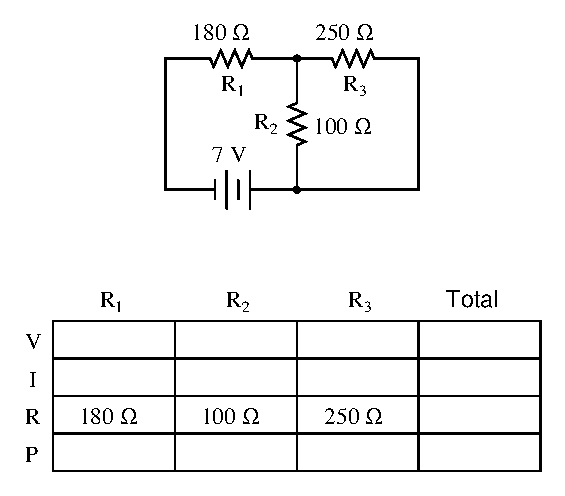
\includegraphics[width=15.5cm]{i01168x01.eps}$$

Når du løser denne oppgaven, bør du lagre alle mellomregninger (dvs. svar fra kalkulatoren som brukes senere i oppgaven) i kalkulatorens minne, slik at du unngår å taste inn verdiene på nytt manuelt. Unødvendig ny inntasting av beregnede verdier introduserer avrundingsfeil i arbeidet, og øker også risikoen for tastefeil. {\it Å unngå unødvendig innføring av feil er et svært viktig prinsipp i instrumentering!}

Hvis sluttresultatene dine blir avrundet som følge av at du ikke gjør dette, får du bare halv uttelling. Dette er en generell praksis for alt matematisk arbeid i dette programmet, ikke bare for denne oppgaven!

\vfil 

Merk: analyse av ethvert serie-parallelt motstandsnettverk blir betydelig enklere med metoden som beskrives i nettboken {\it Lessons In Electric Circuits}, i kapitlet ``Series-Parallel Combination Circuits''.  Der vises en teknikk for å redusere et komplekst serie-parallellnettverk trinn for trinn til én ekvivalent motstand.  Etter denne reduksjonen brukes Ohms lov og Kirchhoffs spennings- og strømlover mens kretsen ``utvides'' tilbake til sin opprinnelige form.  Selv om strømnotasjonen i denne boken bruker elektronflyt i stedet for konvensjonell strømretning, fungerer analysemetoden for serie-parallellkretser like godt.

\underbar{file i01168}
\eject
%(END_QUESTION)





%(BEGIN_ANSWER)

Dette er en vurderingsoppgave -- ingen svar eller hint er gitt!

%(END_ANSWER)





%(BEGIN_NOTES)

$$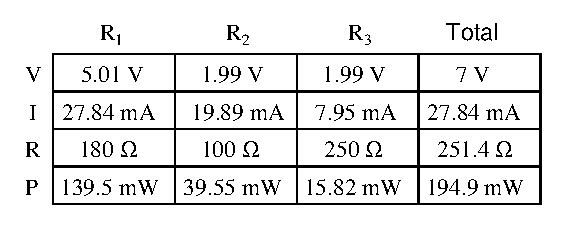
\includegraphics[width=15.5cm]{i01168x02.eps}$$

%(END_NOTES)
